\chapter{Processes}

\section{Process Concept}
\begin{flushleft}
    In modern operating system we want this thing surely:
    \begin{compactitemize}
        \item \textbf{Multi-program}
        \item \textbf{Multi-user}
        \item \textbf{Time-sharing}
    \end{compactitemize}
    Well, the \emph{process} is the abstraction to make it possible.
    
    The program is \emph{passive} entity stored on disk (executable file); process is \emph{active}, so program becomes process when an exacutable file is loaded into memory. One program can be several processes, just consider users executing the same program.
    Each process is identified by a integer number, and two processes must have two difference pids.\\
    
    Process execution must progress in sequential fashion, meaning there is no parallel execution of instructions within a single process. Each instruction is executed one after another in the order determined by the program flow and control structures.
    
    A process consists of multiple components that together define its complete state and execution context:
    \begin{compactitemize}
        \item \textbf{Program code (text section):} Contains the executable instructions that define what the process does
        \item \textbf{Current activity:} Encompasses the program counter and processor registers storing immediate working data
        \item \textbf{Stack:} Contains temporary data such as function parameters, return addresses, and local variables
        \item \textbf{Data section:} Contains global variables that persist throughout the program's execution
        \item \textbf{Heap:} Contains memory that is dynamically allocated during runtime
    \end{compactitemize}
\end{flushleft} 

\begin{figure}[H]
    \centering
    \begin{minipage}{0.2\textwidth}
        \centering
        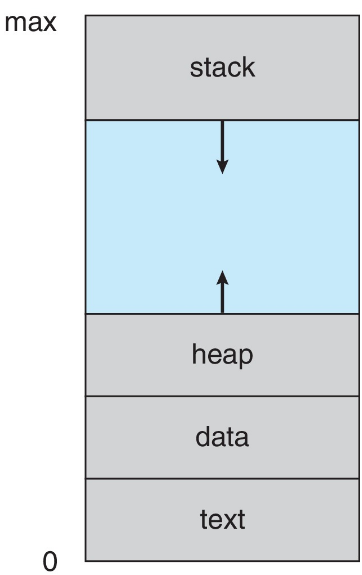
\includegraphics[width=\textwidth]{images/Process_in_memory.png}
        \caption{Process in Memory}
        \label{fig:Process_in_Memory}
    \end{minipage}
    \hfill
    \begin{minipage}{0.7\textwidth}
        \centering
        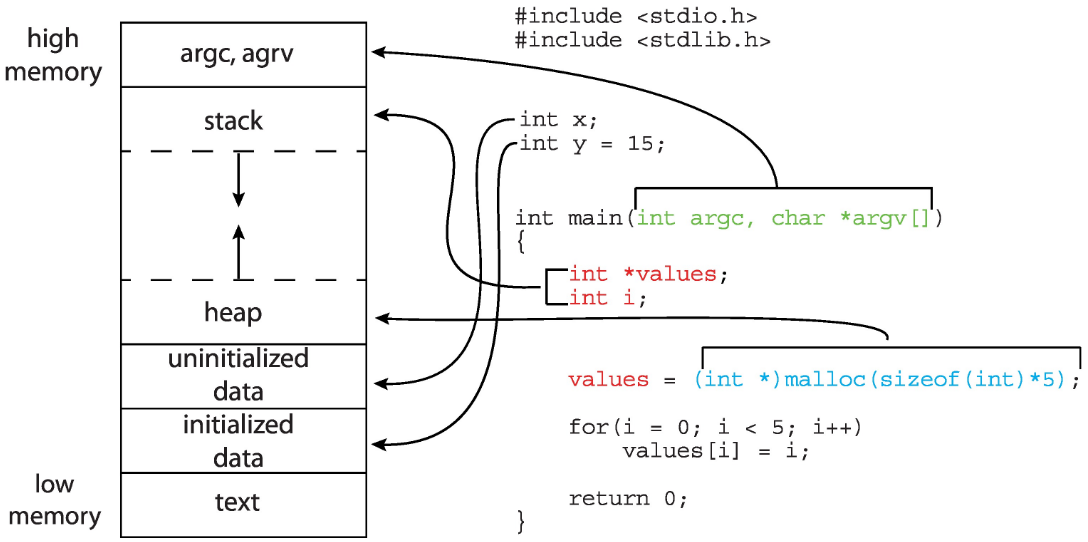
\includegraphics[width=\textwidth]{images/Memory_layout_of_C_program.png}
        \caption{: Memory Layout of C Program}
        \label{fig:memory_layout_of_a_C_program}
    \end{minipage}
    \label{fig:memory_layout_of_a_c_program}
\end{figure}

\section{Process State}
\begin{flushleft}
    A process can be in a differrent state, that possible state changed by OS, but the principal are:
    \begin{compactitemize}
        \item \textbf{New:} The process is being created.
        \item \textbf{Running:} Instructions are being executed.
        \item \textbf{Waiting:} The process is waiting for some event to occur.
        \item \textbf{Ready:} The process is waiting to be assigned to a processor.
        \item \textbf{Terminated:} The process has finished execution.
    \end{compactitemize}
\end{flushleft}

\begin{figure}[H]
    \centering
    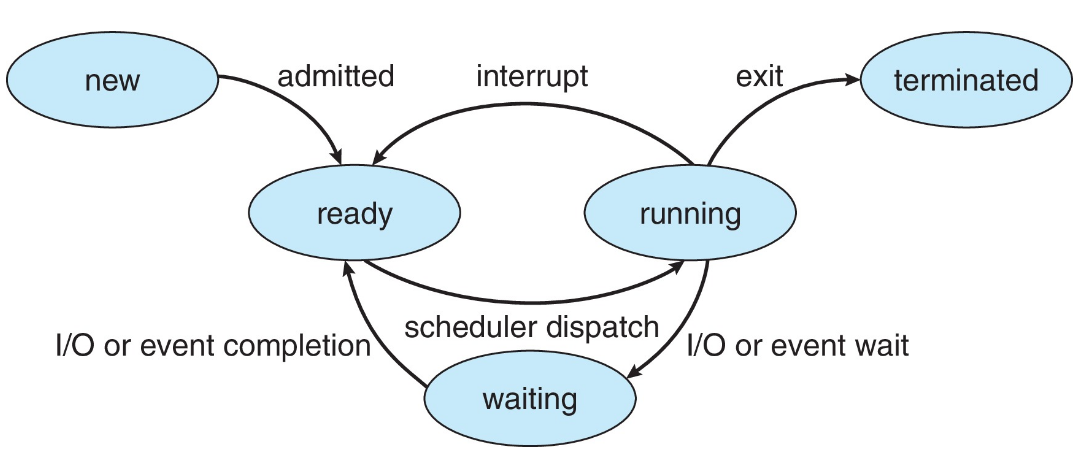
\includegraphics[width=0.7\textwidth]{images/process_states.png}
    \caption{Process States}
    \label{fig:Process States}
\end{figure}

\begin{flushleft}
    In linux other states are present:
    \begin{compactitemize}
        \item \textbf{TASK-INTERRUPTIBLE:} Task is waiting and the wait can be interrupted by signals (a primitive of IPC).
        \item \textbf{TASK-UNINTERRUPTIBLE:} Task is waiting and the wait cannot be interrupted by signals.
        \item \textbf{TASK-STOPPED:} Task execution has been stopped, usually by receiving a signal, or by a terminal action (Ctrl+Z).
        \item \textbf{TASK-TRACED:} The task is traced by another process (e.g a debugger) for step-by-step execution.
        \item \textbf{EXIT-ZOMBIE:} The process is terminated, but its resources have not yet been deallocated. The process creator can still access its return state.
        \item \textbf{EXIT-DEAD:} The process is completely terminated, and all its resources have been deallocated.
    \end{compactitemize}
\end{flushleft}

\section{Process Control Block (PCB)}
\begin{flushleft}
    The PCB is a data structure used by the operating system to store all the information about a process. It is also known as a process descriptor or task control block (TCB). The PCB contains all the information needed to manage and control the execution of a process, including:
    \begin{compactitemize}
        \item \textbf{Process ID (PID):} A unique identifier for the process.
        \item \textbf{Process State:} The current state of the process (e.g., running, waiting, ready).
        \item \textbf{Program Counter (PC):} The address of the next instruction to be executed.
        \item \textbf{CPU Registers:} The values of the CPU registers when the process is not running.
        \item \textbf{Memory Management Information:} Information about the memory allocated to the process, such as base and limit registers, page tables, or segment tables.
        \item \textbf{Accounting Information:} Information about the CPU usage, memory usage, and other resource usage statistics for the process.
        \item \textbf{I/O Status Information:} Information about the I/O devices allocated to the process and their status.
        \item \textbf{List of Open Files:} A list of files that are currently open by the process.
        \item \textbf{Process Priority:} The priority level of the process for scheduling purposes.
        \item \textbf{Parent Process ID:} The PID of the parent process that created this process.
    \end{compactitemize}


The PCB is essential for context switching, which is the process of saving the state of a currently running process and loading the state of another process. When a context switch occurs, the operating system saves the current process's PCB and loads the PCB of the next process to be executed. This allows multiple processes to share a single CPU effectively.
    
\end{flushleft}

\begin{figure}[H]
    \centering
    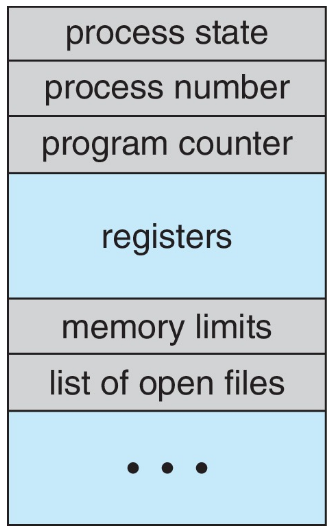
\includegraphics[width=0.2\textwidth]{images/PCB.png}
    \caption{Process Control Block}
    \label{fig:Process Control Block}
\end{figure}

\section{Threads}
